\documentclass[whitelogo]{tudelft-report}
\usepackage{natbib}
\usepackage{fontspec}
\usepackage{changes}
\begin{document}

%% Use Roman numerals for the page numbers of the title pages and table of
%% contents.
\frontmatter

%% Uncomment following 19 lines for a cover with a picture on the lower half only
%\title[tudelft-white]{Title}
%\subtitle[tudelft-cyan]{Optional subtitle}
%\author[tudelft-white]{J.\ Random Author}
%\affiliation{Technische Universiteit Delft}
%\coverimage{cover.jpg}
%\titleoffsetx{10cm}
%\titleoffsety{10cm}
%\afiloffsetx{1cm}
%\afiloffsety{18cm}
%\covertext[tudelft-white]{
%    \textbf{Cover Text} \\
%    possibly \\
%    spanning 
%    multiple 
%    lines
%    \vfill
%    ISBN 000-00-0000-000-0
%}
%\makecover

%% Uncomment following 16 lines for a cover with a picture on the lower half only
\title[tudelft-white]{Luchthaven Schiphol}
\subtitle[tudelft-black]{Issuepaper}
\author[tudelft-white]{C. Wauters}
\affiliation{Technische Universiteit Delft}
\coverimage{SchipholPierPic.jpg}
\covertext[tudelft-white]{
    \textbf{Thema} \\
   Problemen binnen de terminal van een overbelast Schiphol
    \vfill
}
\setpagecolor{tudelft-cyan}
\makecover[split]


%% Include an optional title page.
\begin{titlepage}


\begin{center}

%% Insert the TU Delft logo at the bottom of the page.

%% Print the title in cyan.
{\makeatletter
\largetitlestyle\fontsize{32}{94}\selectfont\ Problemen binnen de terminal van een overbelast Schiphol
%\largetitlestyle\color{tudelft-cyan}\Huge\@title
\makeatother}

%% Print the optional subtitle in black.
{\makeatletter
\ifx\@subtitle\undefined\else
    \bigskip
   {\tudsffamily\fontsize{22}{32}\selectfont\ Issuepaper}    
    %\titlefont\titleshape\LARGE\@subtitle
\fi
\makeatother}

\bigskip
\bigskip

%by
door

\bigskip
\bigskip

%% Print the name of the author.
{\makeatletter
%\largetitlefont\Large\bfseries\@author
\largetitlestyle\fontsize{26}{26}\selectfont\ Casper Wauters
\makeatother}

\bigskip
\bigskip

%to obtain the degree of Master of Science
ter verkrijging van het Bachelors diploma Techniek Bestuur en Management 

%at the Delft University of Technology,
aan de Technische Universiteit Delft,

%to be defended publicly on Tuesday January 1, 2013 at 10:00 AM.
%in het openbaar de verdedigen op dinsdag 1 januari om 10:00 uur.
\begin{figure}[h]
	\centering
	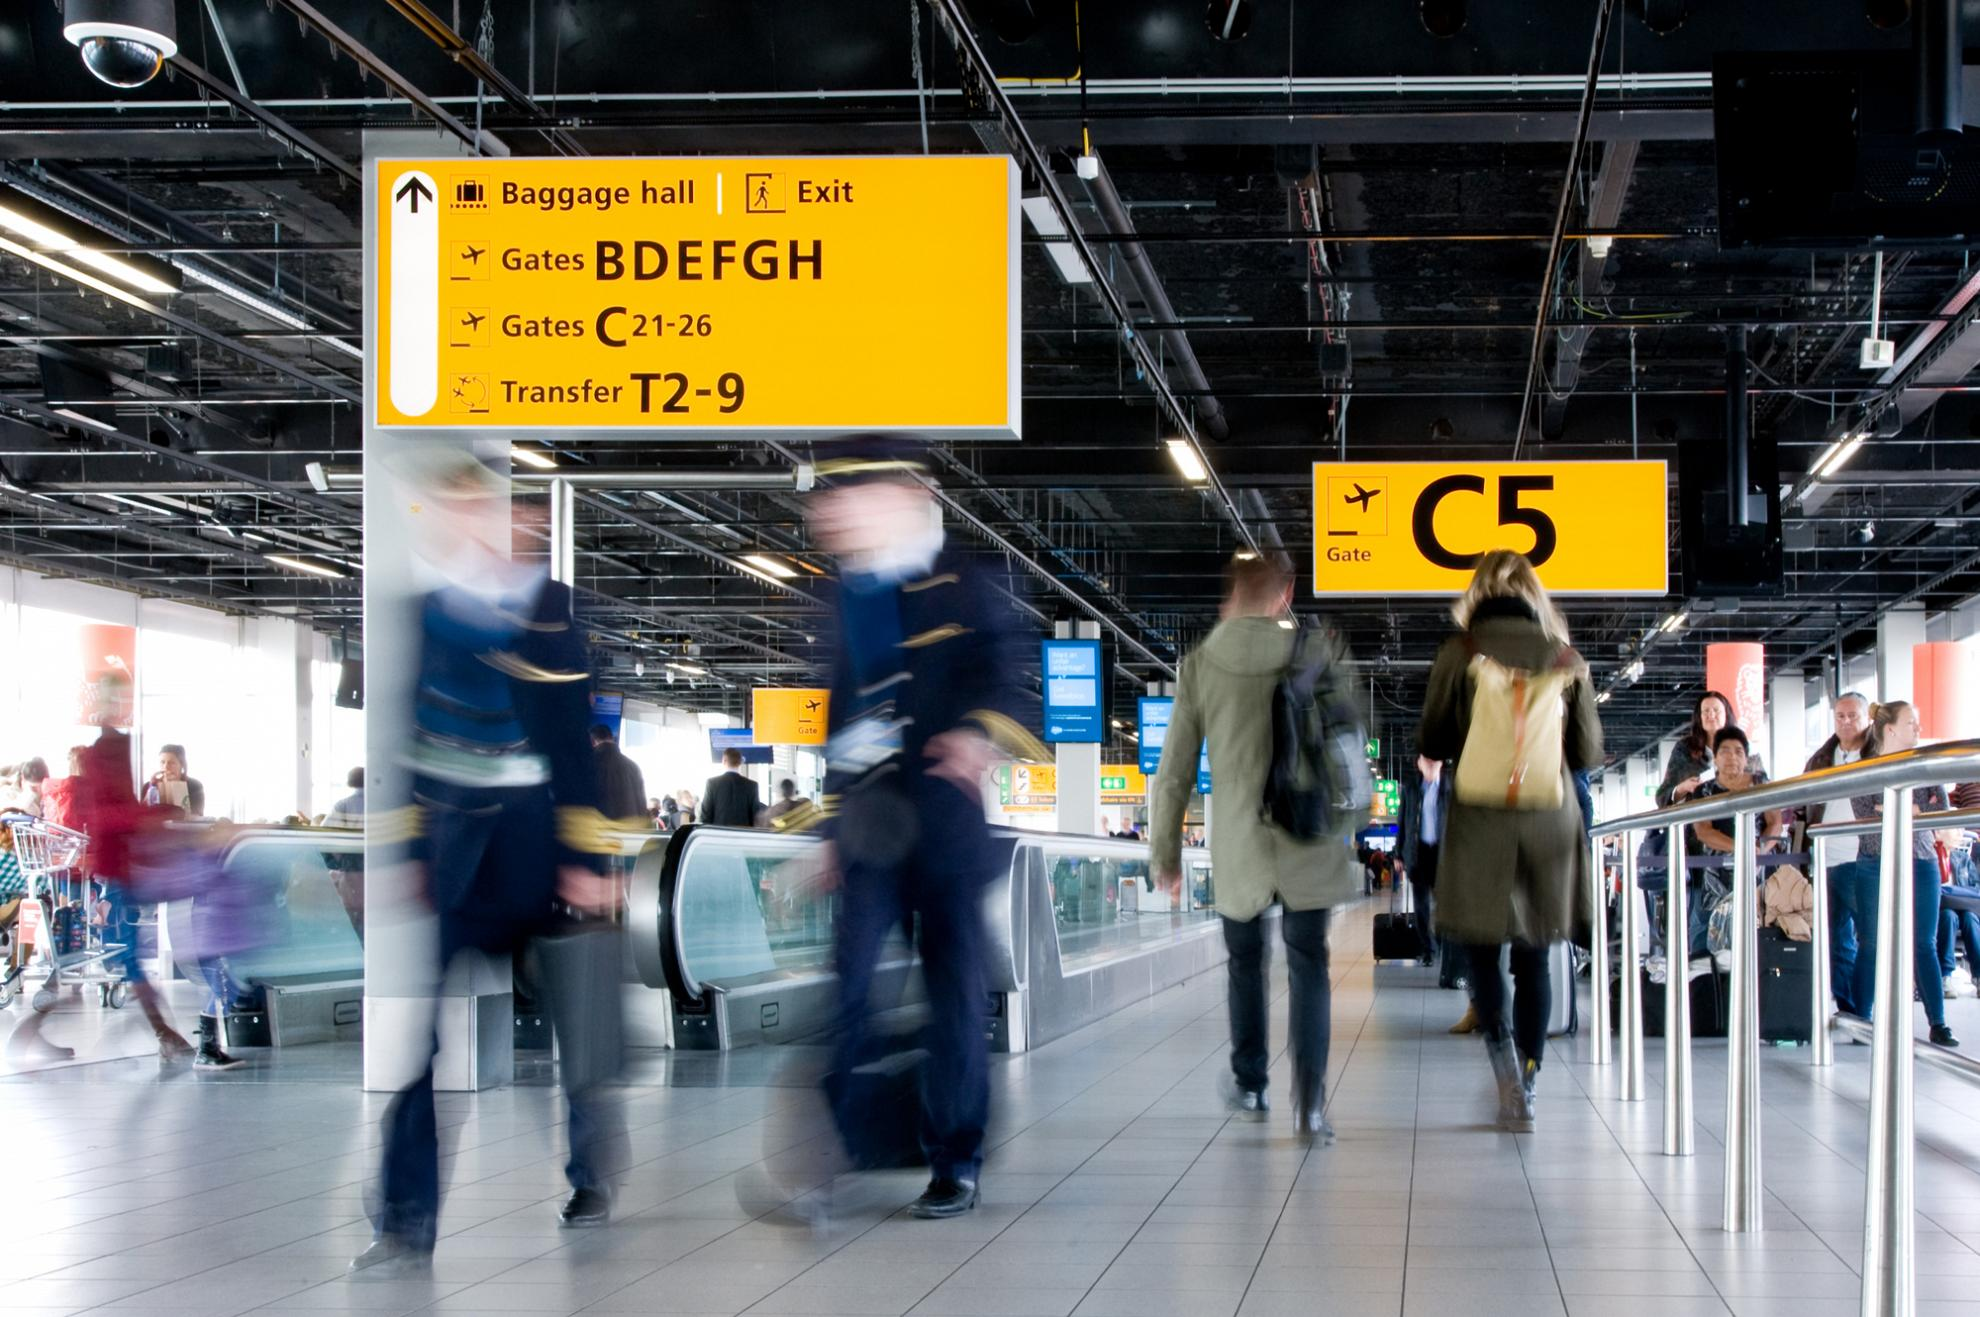
\includegraphics[width=0.9\linewidth]{../../SchipholPierPic}
	\caption{}
	\label{fig:schipholpierpic}
\end{figure}

\vfill

\begin{tabular}{lll}
    Student number: & 1329154 \\
    Begeleiders: & Dr.\ P. Bots, & TU Delft, begeleider \\
        & Dr.\ Ir.\ T.\ Ruijgh-van der Ploeg, & TU Delft, BEP coordinator \\
\end{tabular}
%% Only include the following lines if confidentiality is applicable.

\bigskip
\bigskip
%\emph{This thesis is confidential and cannot be made public until December 31, 2013.}
\emph{Op dit verslag is geheimhouding van toepassing tot en met 31 december 2022.}

\bigskip
\bigskip
%An electronic version of this thesis is available at \url{http://repository.tudelft.nl/}.
%\\[1cm]

%\centering{
\includegraphics{cover/logo_black}}


\end{center}

\begin{tikzpicture}[remember picture, overlay]
    \node at (current page.south)[anchor=south,inner sep=0pt]{
        
\includegraphics{cover/logo_black}
    };
\end{tikzpicture}

\end{titlepage}



\chapter*{Voorwoord}
\setheader{Preface}

In dit issuepaper wordt een analyse gemaakt rondom de problemen van een overbelaste Schipholterminal. Het onderzoek is verricht door een student van Technische Bestuurskunde aan de TU Delft in het kader van zijn Bachelor Eind Project (BEP). 
\\ \\
Het Bachelor eind project is uitgevoerd in samenwerking memt het wayfinding bedrijf Mijksenaar. De Schiphol luchthaven dient als test ‘case’ voor de te onderzoeken theoretische vraagstelling.
\\ \\ 
Allereerst wil ik graag Dr. Pieter Bots en Dr. Ir. Tineke Ruijgh-van der Ploeg hartelijk bedan-ken voor de enthousiaste begeleiding en waardevolle feedback tijdens het eerste fase traject van mijn BEP. Daarnaast wil ik ook mijn dank uitspreken naar het hele Mijksenaar team en in het bijzonder Herbert Sevink en Rijk Boerma. Tot slot nog dank aan mervrouw Spriens-ma voor haar bereidheid tot samenwerking en levering van de nodige Schiphol data.
\\ \\
Namens de auteur,
\\ \\
Casper Wauters






\tableofcontents

%% Use Arabic numerals for the page numbers of the chapters.
\mainmatter

\chapter{Introductie}

\section{Situatieschets}
De Europese luchtvaartmarkt kent de afgelopen 20 jaar een geleidelijk deregulering vanwege drie Europese liberaliseringspaketten (Button et al., 1998). Deze deregulering had als grote pijler om luchtvaartmaatschappijen vrije toegang tot alle luchthavens te verlenen en zo vrije marktwerking te stimuleren. Een aantal belangrijke effecten van deze deregulering wordt in de volgende paragrafen toegelicht.
\subsection{Van ‘point-to-point’ naar ‘hub-and-spoke’}
Daar waar voeger beperkingen werden opgelegd welke luchtvaartmaatschappij recht had op toegang tot specifieke luchthavens, kan een luchtvaartmaatschappij nu naar elke luchthaven een vliegroute openen, indien hij de marktprijs ervoor betaalt. Door het openstellen van de luchthavens zijn vele luchtvaartmaatschappijen hun netwerken gaan herstructureren om nieuwe economische voordelen te creëren. Veel grote spelers hebben hun netwerk veranderd van een ‘point-to-point’ naar ‘hub-and-spoke’ model (Cook \& Goodwin, 2008). Zo werden vluchten naar middelgrote luchthavens vervangen door indirecte vluchten via enkele grote hub-luchthavens. Door het vliegen via een hub-luchthaven kan een luchtvaartmaatschappij veel meer (weliswaar indirecte) bestemmingen aanbieden met minder vluchten (Veldhuis, 2015). Deze hub-luchthavens verkrijgen hierdoor een relatief groot aandeel transferpassagiers. Deze twee strategieën staan in figuur 1.1 gevisualiseerd. \\
\begin{figure}[h]
	\centering
	\includegraphics[width=0.7\linewidth]{screenshot001}
	\caption{visualisatie van ‘point-to-point’ en ‘hub-and-spoke’ strategie (Rodrigue, Comtois, \& Slack, 2013)}
	\label{fig:screenshot001}
\end{figure}
\subsection{Hogere piekbelasting op luchthavens}
Deze ‘shift’ in het businessmodel van luchtvaartmaatschappijen verandert de netwerkkenmerken van de luchtvaart, waarbij tijdelijk verhoogde concentraties een vooraanstaand probleem vormen (Reynolds-Feighan, 2001). Wegens kostenbesparingen en beperkte ‘runway slots’ groeit het gemiddelde aantal stoelen per vliegtuig op een hub-luchthaven (Pagliari, 2007). Een luchthaven heeft nu niet alleen meer reizigers, maar er is ook een verandering van de aankomstintensiteit van reizigers (Werkgroep, 2016). Daarnaast willen luchtvaartmaatschappijen de aansluiting tussen hun hub-vluchten versterken met zo weinig mogelijk wachttijd ertussen. Zo zijn er momenten op de dag waarbij veel hub-vluchten tegelijk aankomen, die een grote hoeveelheid reizigers over een korte tijdsspan generen, denk aan een airbus A380 die ineens tussen de 500 en 800 passagiers (Airbus, 2016) in de luchthaven aflevert en vervolgens ophaalt (Ruehle et al., 2006). Daar waar vroeger het komen en gaan van passagiers een meer evenredige verdeling kende, door de vele klein rechtstreekse vluchten, ontstaat er nu meer een zaagtand verdeling gedurende de dag (ICAO, 2007). Zo krijgen hub-luchthavens niet alleen te maken met meer reizigers via hun terminal, maar ook met hogere piekbelastingen (Burghouwt \& De Wit, 2005).
\begin{figure}[h]
	\centering
	\includegraphics[width=0.7\linewidth]{screenshot002}
	\caption{Ontwikkeling aantal passagier op Schiphol en regionale luchthavens (CBS, 2016)}
	\label{fig:screenshot002}
\end{figure}
De herindeling van het luchtverkeersnetwerk heeft vluchten goedkoper gemaakt (FAA, 1999) en door het economische herstel, na de economische crisis van 2008, hebben reizigers meer koopkracht verkregen. Deze combinatie vormt de perfecte formule voor exponentiële groei in de vraag naar luchtvaart. Sinds 2009 zien de Nederlandse luchthavens deze groei elk jaar opnieuw doorzetten. Figuur 1.2 laat deze ontwikkeling zien per kwartaal tussen 2012 en 2015 in percentage-mutatie t.o.v. een jaar eerder (CBS, 2016).
\\ \\
Door deze aanhoudende groei ontstaat er een onbalans tussen de beschikbare luchthavencapaciteit en de vraag van het luchtverkeer op het huidige systeem. De luchthavens zijn vanuit vroeger niet op de nieuwe luchtverkeerspatronen ontworpen en moeten tegelijkertijd aan de sterke marktgroei voldoen, waardoor compromissen bereikt moeten worden (Hamzawi, 1992; Forsyth, 2007). De huidige indeling van de faciliteiten is niet ideaal voor hub-verkeer en heeft een negatieve invloed op de verdiensten. Een goed voorbeeld is de bezetting van de pieren; op piekmomenten ontstaat congestie op de pieren en op dal momenten zijn er leegstaande pieren met onbenutte zitplaatsen en retail faciliteiten.
\subsection{Lager dan verwachtte inkomsten}
Van de kernpunten van een luchthaven die gewaarborgd moeten worden, zijn de luchthaven operaties en ‘retail’\footnote{Retail: Betreft het verkoopproces van producten of diensten naar de consument via verkoopkanalen als winkels en horeca voor het genereren van inkomsten.}  het meeste aan verandering onderhevig. Het beleid vanuit het bestuur van een luchthaven verandert qua focus tussen de luchthaven operaties en retail, afhankelijk van kansen en noodzaak. Door de evolutie van de markt vindt de afgelopen jaren vooral een verschuiving richting de operaties van de luchthaven plaats, meer specifiek de verwerking van het groeiend aantal passagiers en vliegtuigen, en wordt minder aandacht besteed aan de retail zijde van de luchthaven.
\begin{figure}[h]
	\centering
	\includegraphics[width=0.7\linewidth]{screenshot003}
	\caption{Omzet Nederlandse luchtvaart (CBS, 2016)}
	\label{fig:screenshot003}
\end{figure}
Door de gekozen prioriteiten van het Schiphol bestuur is in deze tijden van economische herstel het exploitatieresultaat niet in verhouding toegenomen. Een belangrijke factor hierin is de tegenvallende cijfers van de retail gerelateerde inkomsten (zo genoemde consumer products \& services). Zo zijn de bestedingen per passagier op Schiphol gedaald van €15,89 in 2013 naar €14,45 in 2015 (Schiphol Group, 2016). Deze daling in bestedingen is van groot belang voor het exploitatieresultaat. Uit het jaarverslag van Schiphol is zichtbaar dat na aftrek van kosten de inkomsten uit de vliegactiviteiten maar zeer beperkt bijdragen aan de bedrijfswinst (zie figuur 1.4 voor de balans uit het jaarverslag van 2015).
\\ \\
\begin{figure}[h]
	\centering
	\includegraphics[width=0.7\linewidth]{screenshot004}
	\caption{Kerncijfers uit het jaarverslag van Schiphol (2015). Activiteiten avaiation versus consumer products \& services (Schiphol Group, 2016)}
	\label{fig:screenshot004}
\end{figure}
Schiphol weet het groeiend aantal passagiers steeds slechter te bereiken met zijn retail. Met de huidige indeling van de terminal zit een groot deel van de passagiers bij de gate te wachten waar opvallend weinig retail wordt aangeboden en hier worden veel potentiële inkomsten misgelopen. Veel transfer passagiers worden zodanig rondgeleid dat ze zich van pier naar pier verplaatsen en daarbij het lounge gebied van de terminal niet doorkruisen. Het resultaat is dat een groot deel van de passagiers zitten te wachten bij een kiosk of klein cafetaria op de pier. Vooralsnog wordt een groot deel van de passagiers niet goed bediend, met weinig prikkels tot koopgedrag wegens het gebrek aan bereik en diversiteit. (H. Seevinck, Mijksenaar, personal communication, 2015).
\pagebreak
\section{Onderzoeksdoel}
Luchthavenoperaties en retail leveren een constant spanningsveld op qua prioriteit. Strategische keuzes moeten worden gemaakt om beide elementen te balanceren. Voor het Schiphol bestuur is de vraag, zijn er ‘opportunity windows’\footnote{Een opportunity window is een periode in de tijd waarbij acties kunnen worden ondernomen voor een gewenste uitkomst. Wanneer deze specifieke periode in de tijd is verlopen, is de gewenste uitkomst niet meer mogelijk}  waarbij een verschuiving in focus mogelijk is, of zijn er nieuwe invalshoeken die beide aspecten bedienen?
\\ \\
Met het in acht nemen van bovenstaande situatie richt dit paper zich op de herstructurering van luchthaven Schiphol en zijn middelen. De afbakening en identificatie van de spanning tussen middelen kan herschreven worden tot de volgende probleemstelling:
\begin{quote}
    \textbf{Hoe kan Schiphol de huidig beschikbare middelen herstructureren om zo vanuit de passagiersstromen een commercieel hoger rendement te behalen, zonder dat de operaties in het geding komen?}
\end{quote}
Allereerst zal in hoofdstuk 2 de probleemanalyse worden beschreven, deze berust op verschillende deelanalyses welke te vinden zijn in de bijlage van dit document. Er wordt inzicht gegeven in de middelen die een luchthavenbestuur tot zijn beschikking heeft om zich naar de gewenste situatie te bewegen. Een luchthaven bestaat uit een complex web van verschillende actoren die in dit hoofdstuk worden toegelicht. Vervolgens wordt in hoofdstuk 3 een onderzoeksrichting gegeven aan de hand van kennislacunes en wordt een voorstel tot onderzoek naar de ontbrekende kennis opgesteld.
\chapter{Probleemanalyse}






%% Use letters for the chapter numbers of the appendices.
\appendix

%\input{appendix-a}

\bibliography{report}

\end{document}

